\chapter{Systemidentifikation im Zeitbereich}
\todo[inline]{kurze Einleitung schreiben}

\section{\textit{Least Squares}-Methode}
In diesem Kapitel wird die Methode der kleinsten Fehlerquadrate (\textit{Least Squares}, LSQ) vorgestellt.
Eine der Kernaufgaben vieler Ingenieure besteht darin, einen belastbaren Zusammenhang zwischen gemessenen Werten zu finden. 
Diese Zusammenhänge können näherungsweise durch folgendes lineares Modell beschrieben werden:  
\begin{equation}
    z = H\cdot x+v 
\end{equation}
mit 
\begin{align}
	\begin{split}
		\text{Messvektor: } &\dim{(z)} = m\times 1\\
		\text{bekannte Matrix: } &\dim{(H)} = m\times n\\
		\text{unbekannter Rauschterm: } &\dim{(v)} = m\times1\\
		\text{unbekannter Parametervektor: } &\dim{(x)} = n\times 1
		\nonumber
	\end{split}
\end{align}

Die LSQ-Methode kann beispielsweise verwendet werden, um die Schätzung von Modellparametern im Rahmen der 
Systemidentifikation durchzuführen. Gesucht ist dabei ein Schätzwert $\hat{x}$ für den Parametervektor. Der Restfehlervektor 
$e$ lautet:
\begin{equation}
    e = z - H\cdot \hat{x} \\
\end{equation}

Die Idee besteht darin, einen Wert von $\hat{x}$ zu finden, der die Norm des quadrierten Restfehlervektors minimiert. Das 
quadratische Zielfunktional $J$ ist gegeben durch: 
\begin{align}
   \begin{split}
     J &= \frac{1}{2} \cdot e^{T} \cdot e \\
     &= \frac{1}{2} \cdot {(z- H\hat{x})}^{T}\cdot(z- H\hat{x}) \\
     &= \frac{1}{2} \cdot (z^{T} -{\hat{x}}^{T}H^{T})\cdot(z- H\hat{x}) \\
     &= \frac{1}{2} \cdot z^{T}z - z^{T}H\hat{x} + \frac{1}{2}\cdot {\hat{x}}^{T}A\hat{x}  \\
   \end{split}
\end{align}
mit $A = H^{T}H$. Die Lösung des Minimierungsproblems lautet dann:
\begin{equation}
    \hat{x}= {(H^{T} H)}^{-1} \cdot H^{T} z 
\end{equation}


\subsection{Schätzung der Parameter mit dem LSQ-Verfahren} 

Die Zustandsraumdarstellung \eqref{eq:laengsbewegung} liefert folgende Gleichungen: 

\begin{align}
	\Delta\dot \alpha-q &=  \frac{Z_{\alpha}\Delta\alpha}{V_0} + \frac{Z_{\nu}\Delta V_{A}}{V_0} + 
	\frac{Z_{\eta}\Delta\eta}{V_0} - \frac{X_{\delta_F}\sin{(\alpha_0)}\cdot\Delta\delta_F}{V_0}\\
	\dot q &= M_{\alpha}\Delta\alpha + M_q q + M_{\nu}\Delta V_A + M_{\eta}\Delta\eta + M{\delta_F}\Delta\delta_F\\
	\Delta\dot V_A &= X_{\alpha}\Delta\alpha +  X_{\nu}\Delta V_A + X_{\eta}\Delta\eta + 
	X_{\delta_F}\cos{(\alpha_0)}\cdot\Delta\delta_F \\
	\Delta \dot \gamma &= \frac{- Z_{\alpha}\Delta\alpha}{V_0} + \frac{- Z_{\nu}\Delta V_{A}}{V_0} + 
	\frac{-Z_{\eta}\Delta\eta}{V_0} + \frac{X_{\delta F}\sin{(\alpha_0)}\cdot\Delta\delta_F}{V_0}
\end{align}
	
Diese können zu einem linearen Gleichungssystem umgeformt werden: 
\begin{equation}
    z_{L}= H_{L}\cdot x + v
\end{equation}

Die einzelnen Vektoren und Matrizen lauten:
\setcounter{MaxMatrixCols}{15}
\begin{equation}
	z_{L} = (\Delta\dot \alpha-q \;\; \dot q \;\; \Delta\dot V_A)^T
\end{equation}

\begin{equation}
	 H_{L} = \begin{pmatrix}
		0&0&0& \frac{-\sin{(\alpha_0)}\cdot\Delta\delta_F}{V_0} & \frac{\Delta\alpha}{V_0}& \frac{\Delta V_A}{V_0} & 
		\frac{\Delta\eta}{V_0} &0&0&0&0&0   \\
		0&0&0&0&0&0&0 &\Delta\alpha & q & \Delta V_A & \Delta\eta & \Delta\delta_F \\
		\Delta\alpha &  \Delta V_A & \Delta\eta & \cos{(\alpha_0)}\cdot\Delta\delta_F &0&0&0&0&0&0&0&0 
	\end{pmatrix}
\end{equation}

\begin{equation}
	x = (X_{\alpha}\; 
	X_{\nu}\;
	X_{\eta}\;
	X_{\delta_F}\; 
	Z_{\alpha}\; 
	Z_{\nu}\;
	Z_{\eta}\;
	M_{\alpha}\;
	M_{q}\;
	M_{\nu}\;
	M_{\eta}\;
	M_{\delta_F})^T \\
\end{equation}  
Wie schon in dem letzten Abschnitt erwähnt, wird es nach einem geschätzten Paramertervektor $\hat{x}$ gesucht, der die Norm des quadrierten Restfehlervektors $ e = z - H\cdot \hat{x}$ minimiert. Die Lösung ist laut (4.4)
\begin{equation}
    \hat{x}= {({H_L}^{T} {H_L})}^{-1} \cdot {H_L}^{T} z_L 
\end{equation}

 
 \section{Ergebnisse}
 
Anschließend werden die Ergebnisse in diesem Kapitel kurz vorgestellt.

Nach der Schätzung der Einträge der Matrizen $A$ und $B$ wird das Anfangswertproblem \eqref{eq:laengsbewegung} im gesamten 
Zeitintervall gelöst. Bei allen Simulationen sind die Filterparametern wie in \ref{section:filterung} gewählt.

In \cref{fig:Ergebnisse_zmlsq} wird die Lösung anhand des Matrix-LSQ-Verfahrens dargestellt. Die geschätzte Matrizen $A_L$ und $B_L$ lauten: 
\begin{equation}
 	A_L = \begin{pmatrix}
 		-0.1940 & 0.005 & -0.0002 & -0.0540 \\
 		-38.9899 & -12.8888 & 0.3632 & -4.2686 \\
 		-6.1506 & -0.1501 & -0.0589 & -5.0107 \\
 		0.4433 & 0.0427 & 0.0023 & 0.0818
 	\end{pmatrix} \;\;\; , \;\;\;
 	A = \begin{pmatrix}
		\frac{Z_\alpha}{V_0} & 1 & \frac{Z_V}{V_0} & 0\\
		M_\alpha & M_q & M_V & 0\\
		X_\alpha & 0 & X_V & -g\\
		-\frac{Z_\alpha}{V_0} & 0 & -\frac{Z_V}{V_0} & 0\\
	\end{pmatrix}
	\nonumber
\end{equation}

\begin{equation}
 	 B_L = \begin{pmatrix}
 		-0.0267 & -0.0164 \\ 
 		-26.1377 & -12.9651 \\
 		-0.7414 & 4.6092 \\
 		0.0477 & -0.1328
 	\end{pmatrix}  \;\;\; , \;\;\;
 	B= \begin{pmatrix}
		\frac{Z_\eta}{V_0} & -\frac{X_{\delta F}}{V_0} \sin{(\alpha_0)}\\
		M_\eta & M_{\delta F}\\
		X_\eta & X_{\delta F} \cos{(\alpha_0)}\\
		-\frac{Z_\eta}{V_0} & \frac{X_{\delta F}}{V_0} \sin{(\alpha_0)}\\
	\end{pmatrix}
 \nonumber
\end{equation}
Die Ergebnisse in \cref{fig:Ergebnisse_zmlsq} zeigen eine relativ präzise Approximation. Allerdings weist das Ergebnis in flugmechanischer 
Hinsicht Abweichungen in System- und Eingangsmatrix auf. Der Betrag der Einträge der ersten und vierten Spalten von $A_L$ unterscheiden sich stark voneinander ($-0.1940$ und $0.4433$) und ($-0.0002$ und $0.0023$). Eine Starke Abweichung ist auch zwischen die vierten Spalten der Matrizen $A_L$ und $A$.  

 
\cref{fig:Ergebnisse_zlsq} zeigt die Lösung anhand des LSQ-Verfahrens. Die Methode liefert keine sonderlich guten Ergebnisse. Der Simulator kann keine stabilen Werten generieren. 

\todo{warum schlechte Ergebnisse? : Adam : ich weiß nicht warum?}
\begin{figure}[h!]
	\centering
	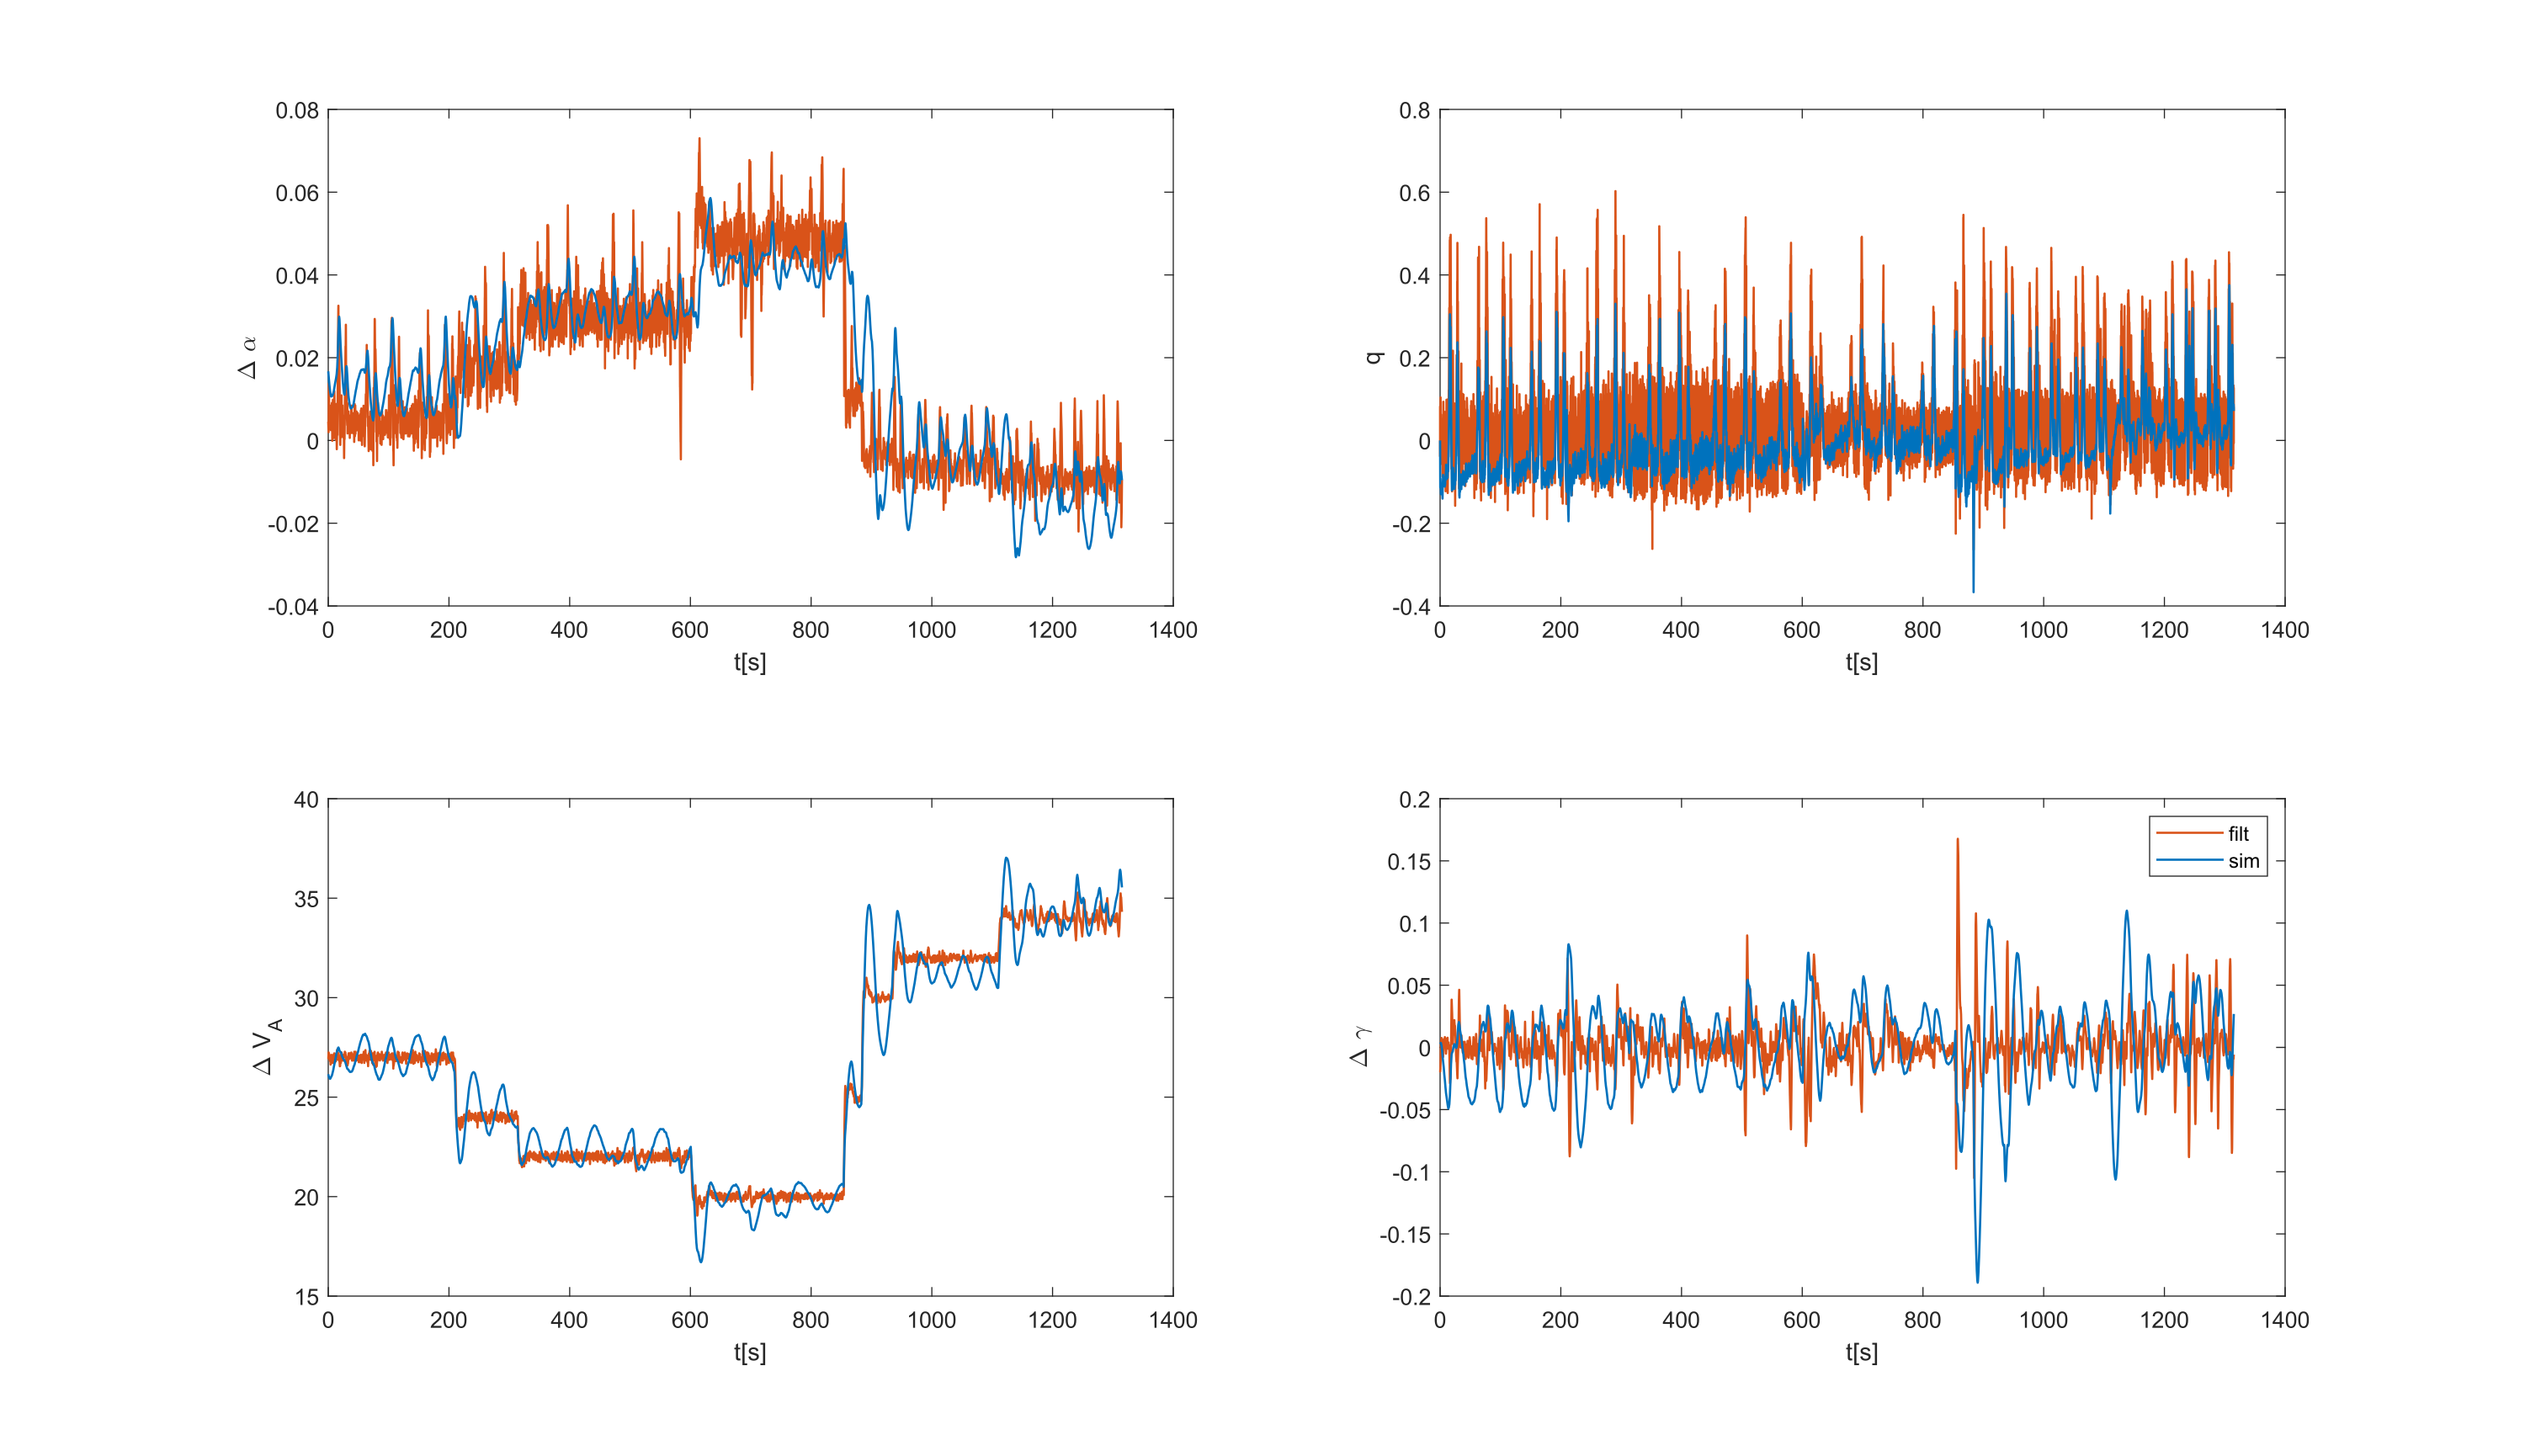
\includegraphics[trim=100 0 100 0,clip,width=1\linewidth]{LS.png}
	\caption{Ergebnisse anhand des Matrix-LSQ-Verfahrens}
    \label{fig:Ergebnisse_zmlsq}
\end{figure}

 \begin{figure}[h!]
	\centering
	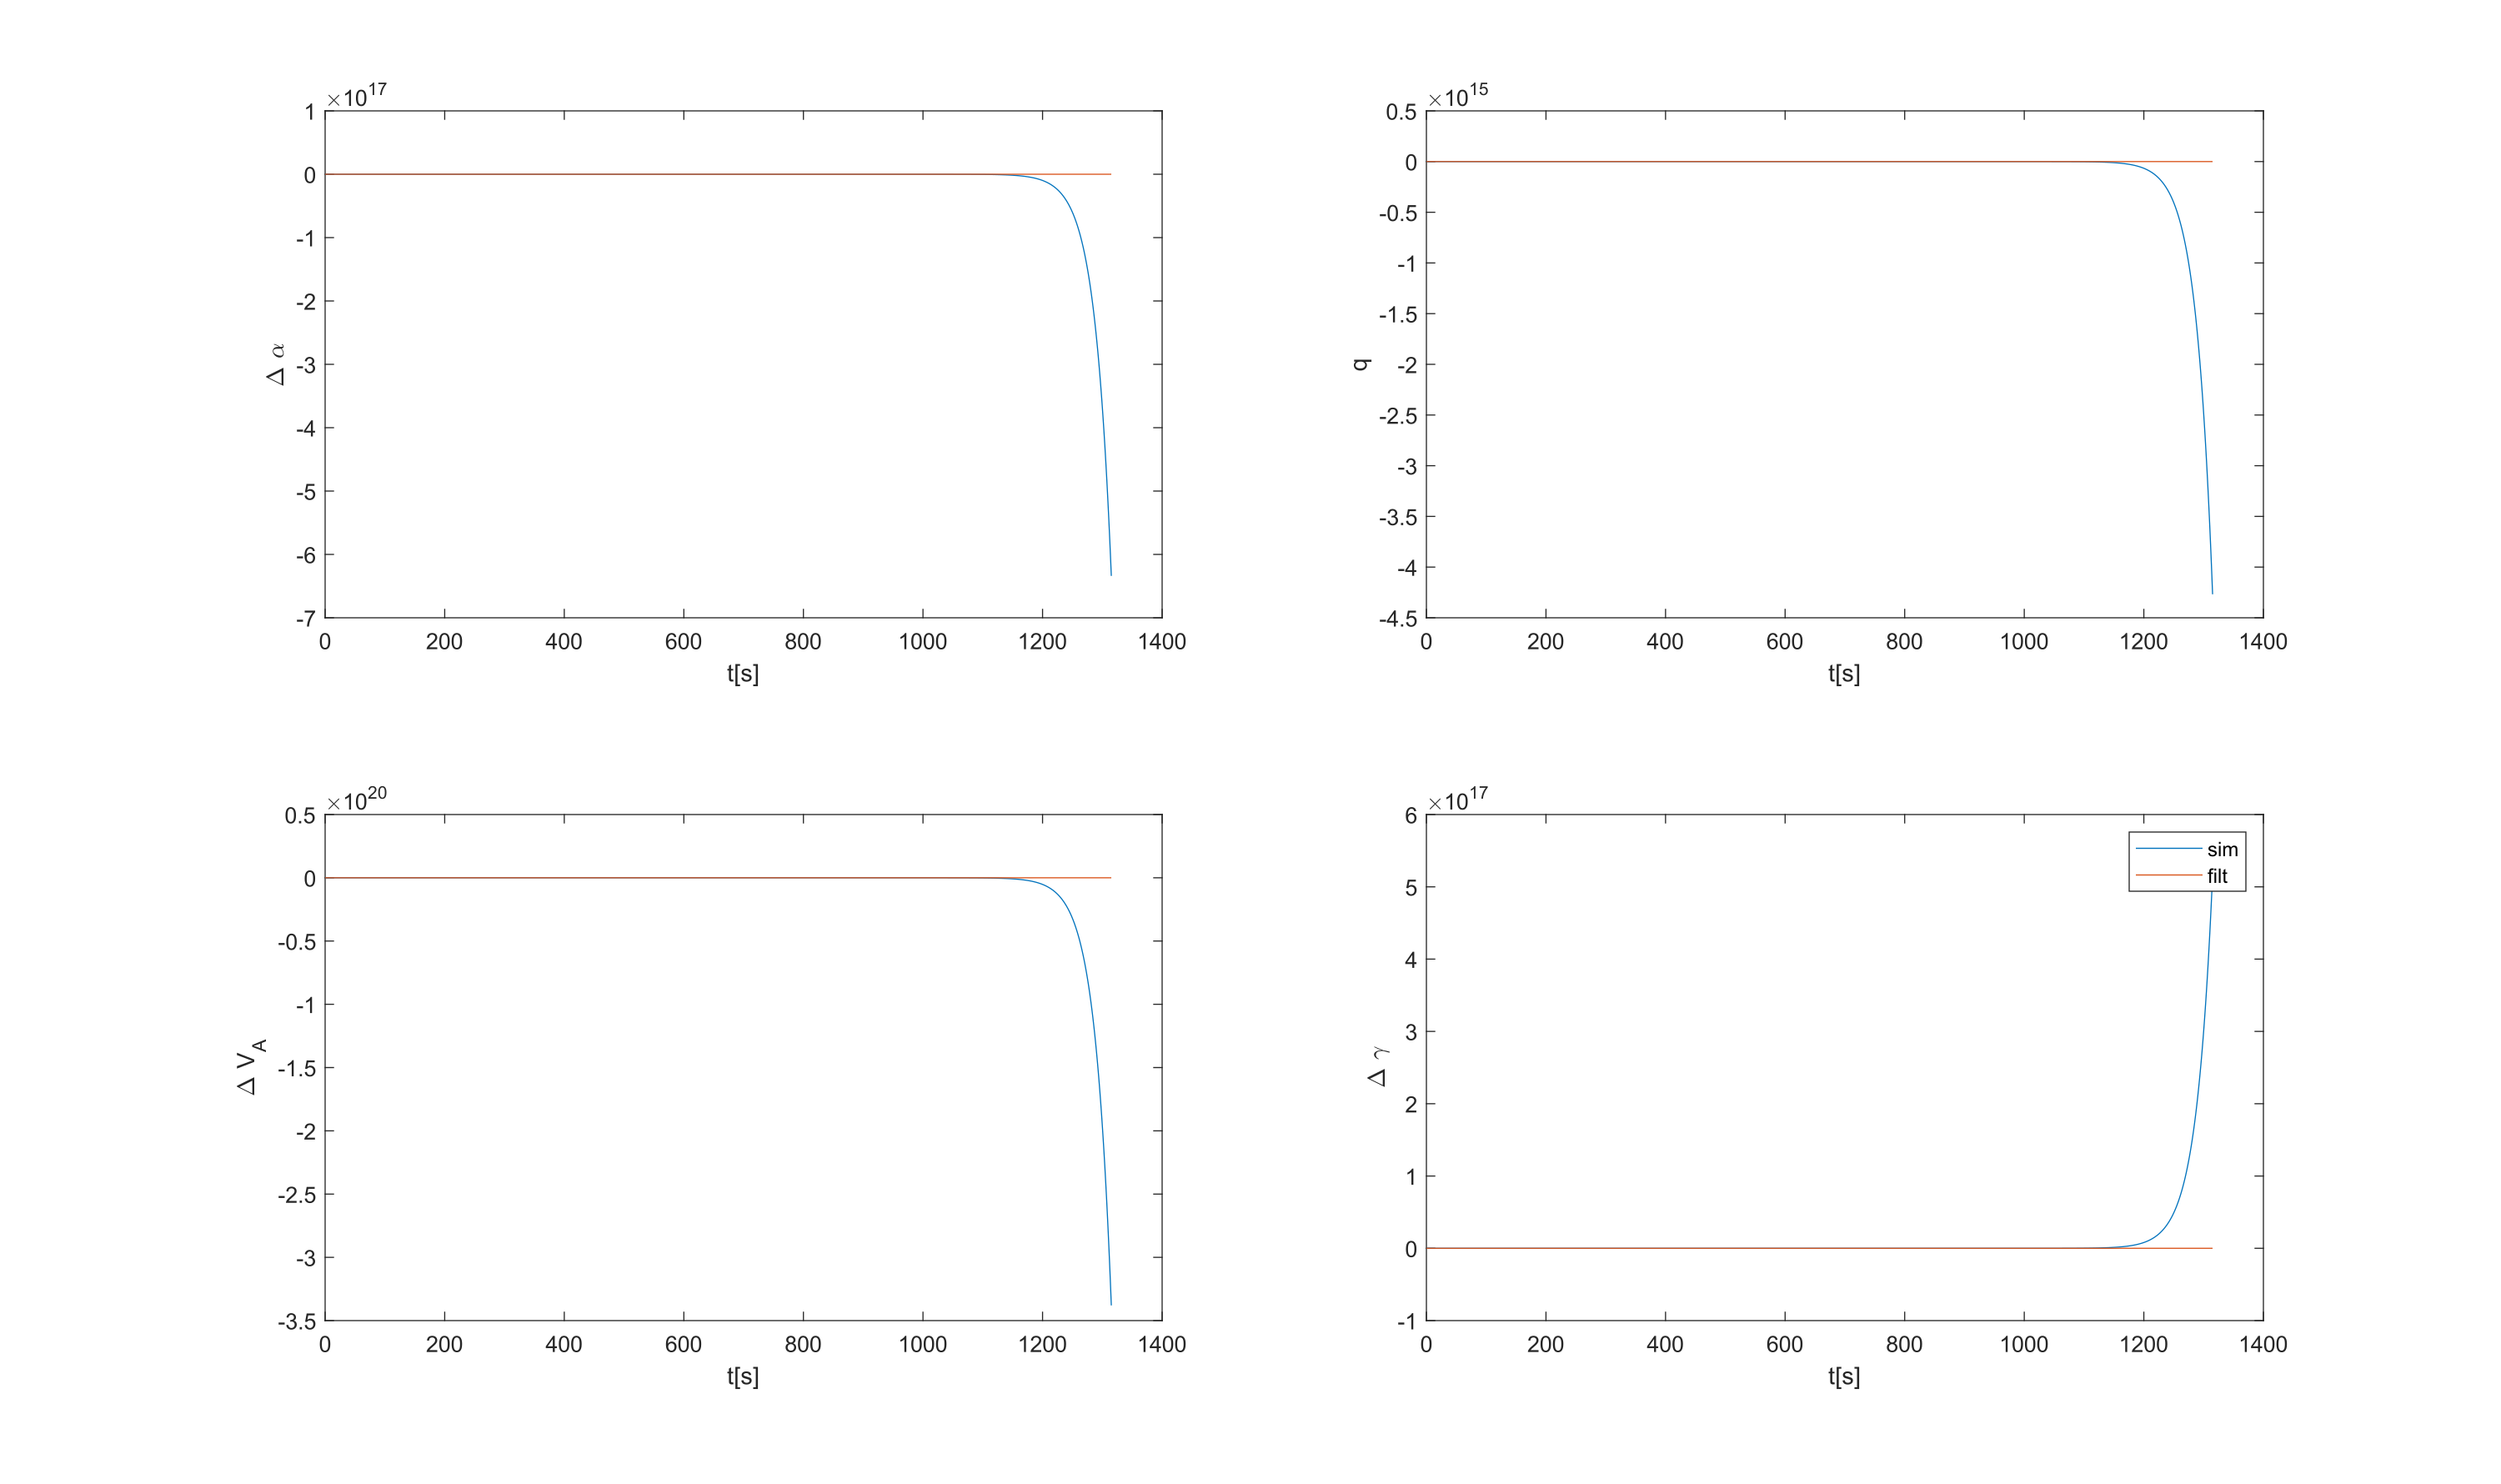
\includegraphics[trim=100 0 100 0,clip,width=1\linewidth]{LS_LSQ.png}
	\caption{Ergebnisse anhand des LSQ-Verfahrens}
     \label{fig:Ergebnisse_zlsq} 
\end{figure}

\todo{Diagramme gut lesbar?}

